\documentclass[ucs,9pt]{beamer}

% Copyright 2004 by Till Tantau <tantau@users.sourceforge.net>.
%
% In principle, this file can be redistributed and/or modified under
% the terms of the GNU Public License, version 2.
%
% However, this file is supposed to be a template to be modified
% for your own needs. For this reason, if you use this file as a
% template and not specifically distribute it as part of a another
% package/program, I grant the extra permission to freely copy and
% modify this file as you see fit and even to delete this copyright
% notice.
%
% Modified by Tobias G. Pfeiffer <tobias.pfeiffer@math.fu-berlin.de>
% to show usage of some features specific to the FU Berlin template.

% remove this line and the "ucs" option to the documentclass when your editor is not utf8-capable
\usepackage[utf8x]{inputenc} % to make utf-8 input possible
\usepackage[english]{babel} % hyphenation etc., alternatively use 'german' as parameter

% Template for talks using the Corporate Design of the Freie Universitaet
%   Berlin, created following the guidelines on www.fu-berlin.de/cd by
%   Tobias G. Pfeiffer, <tobias.pfeiffer@math.fu-berlin.de>
% This file can be redistributed and/or modified in any way you like.
%   If you feel you have done significant improvements to this template,
%   please consider providing your modified version to
%   https://www.mi.fu-berlin.de/w/Mi/BeamerTemplateCorporateDesign

\usepackage{amsmath,dsfont,listings}

%%% FU logo
% small version for upper right corner of normal pages
\pgfdeclareimage[height=0.9cm]{university-logo}{FULogo_RGB}
\logo{\pgfuseimage{university-logo}}
% large version for upper right corner of title page
\pgfdeclareimage[height=1.085cm]{big-university-logo}{FULogo_RGB}
\newcommand{\titleimage}[1]{\pgfdeclareimage[height=2.92cm]{title-image}{#1}}
\titlegraphic{\pgfuseimage{title-image}}
%%% end FU logo

% NOTE: 1cm = 0.393 in = 28.346 pt;    1 pt = 1/72 in = 0.0352 cm
\setbeamersize{text margin right=3.5mm, text margin left=7.5mm}  % text margin

% colors to be used
\definecolor{text-grey}{rgb}{0.45, 0.45, 0.45} % grey text on white background
\definecolor{bg-grey}{rgb}{0.66, 0.65, 0.60} % grey background (for white text)
\definecolor{fu-blue}{RGB}{0, 51, 102} % blue text
\definecolor{fu-green}{RGB}{153, 204, 0} % green text
\definecolor{fu-red}{RGB}{204, 0, 0} % red text (used by \alert)

% switch off the sidebars
% TODO: loading \useoutertheme{sidebar} (which is maybe wanted) also inserts
%   a sidebar on title page (unwanted), also indents the page title (unwanted?),
%   and duplicates the navigation symbols (unwanted)
\setbeamersize{sidebar width left=0cm, sidebar width right=0mm}
\setbeamertemplate{sidebar right}{}
\setbeamertemplate{sidebar left}{}
%    XOR
% \useoutertheme{sidebar}

% frame title
% is truncated before logo and splits on two lines
% if neccessary (or manually using \\)
\setbeamertemplate{frametitle}{%
    \vskip-30pt \color{text-grey}\large%
    \begin{minipage}[b][23pt]{80.5mm}%
    \flushleft\insertframetitle%
    \end{minipage}%
}

%%% title page
% TODO: get rid of the navigation symbols on the title page.
%   actually, \frame[plain] *should* remove them...
\setbeamertemplate{title page}{
% upper right: FU logo
\vskip2pt\hfill\pgfuseimage{big-university-logo} \\
\vskip6pt\hskip3pt
% title image of the presentation
\begin{minipage}{11.6cm}
\hspace{-1mm}\inserttitlegraphic
\end{minipage}

% set the title and the author
\vskip14pt
\parbox[top][1.35cm][c]{11cm}{\color{text-grey}\inserttitle \\ \small \insertsubtitle}
\vskip11pt
\parbox[top][1.35cm][c]{11cm}{\small \insertauthor \\ \insertinstitute \\[3mm] \insertdate}
}
%%% end title page

%%% colors
\usecolortheme{lily}
\setbeamercolor*{normal text}{fg=black,bg=white}
\setbeamercolor*{alerted text}{fg=fu-red}
\setbeamercolor*{example text}{fg=fu-green}
\setbeamercolor*{structure}{fg=fu-blue}

\setbeamercolor*{block title}{fg=white,bg=black!50}
\setbeamercolor*{block title alerted}{fg=white,bg=black!50}
\setbeamercolor*{block title example}{fg=white,bg=black!50}

\setbeamercolor*{block body}{bg=black!10}
\setbeamercolor*{block body alerted}{bg=black!10}
\setbeamercolor*{block body example}{bg=black!10}

\setbeamercolor{bibliography entry author}{fg=fu-blue}
% TODO: this doesn't work at all:
\setbeamercolor{bibliography entry journal}{fg=text-grey}

\setbeamercolor{item}{fg=fu-blue}
\setbeamercolor{navigation symbols}{fg=text-grey,bg=bg-grey}
%%% end colors

%%% headline
\setbeamertemplate{headline}{
\vskip4pt\hfill\insertlogo\hspace{3.5mm} % logo on the right

\vskip6pt\color{fu-blue}\rule{\textwidth}{0.4pt} % horizontal line
}
%%% end headline

%%% footline
\newcommand{\footlinetext}{\insertshortinstitute, \insertshorttitle, \insertshortdate}
\setbeamertemplate{footline}{
\vskip5pt\color{fu-blue}\rule{\textwidth}{0.4pt}\\ % horizontal line
\vskip2pt
\makebox[123mm]{\hspace{7.5mm}
\color{fu-blue}\footlinetext
\hfill \raisebox{-1pt}{\usebeamertemplate***{navigation symbols}}
\hfill \insertframenumber}
\vskip4pt
}
%%% end footline

%%% settings for listings package
\lstset{extendedchars=true, showstringspaces=false, basicstyle=\footnotesize\sffamily, tabsize=2, breaklines=true, breakindent=10pt, frame=l, columns=fullflexible}
\lstset{language=Java} % this sets the syntax highlighting
\lstset{mathescape=true} % this switches on $...$ substitution in code
% enables UTF-8 in source code:
\lstset{literate={ä}{{\"a}}1 {ö}{{\"o}}1 {ü}{{\"u}}1 {Ä}{{\"A}}1 {Ö}{{\"O}}1 {Ü}{{\"U}}1 {ß}{\ss}1}
%%% end listings % THIS is the line that includes the FU template!

\usepackage{arev,t1enc} % looks nicer than the standard sans-serif font
% if you experience problems, comment out the line above and change
% the documentclass option "9pt" to "10pt"

\usepackage{graphicx}

% image to be shown on the title page (without file extension, should be pdf or png)
\titleimage{fu_500}

\title[Short Paper Title] % (optional, use only with long paper titles)
{Title As It Is In the Proceedings}

\subtitle
{Include Only If Paper Has a Subtitle}

\author[Author, Another] % (optional, use only with lots of authors)
{F.~Author \and S.~Another}
% - Give the names in the same order as the appear in the paper.

\institute[FU Berlin] % (optional, but mostly needed)
{Freie Universität Berlin}
% - Keep it simple, no one is interested in your street address.

\date[CFP 2003] % (optional, should be abbreviation of conference name)
{Conference on Fabulous Presentations, 2003}
% - Either use conference name or its abbreviation.
% - Not really informative to the audience, more for people (including
% yourself) who are reading the slides online

\subject{Theoretical Computer Science}
% This is only inserted into the PDF information catalog. Can be left
% out.

% you can redefine the text shown in the footline. use a combination of
% \insertshortauthor, \insertshortinstitute, \insertshorttitle, \insertshortdate, ...
\renewcommand{\footlinetext}{\insertshortinstitute, \insertshorttitle, \insertshortdate}

% Delete this, if you do not want the table of contents to pop up at
% the beginning of each subsection:
\AtBeginSubsection[]
{
  \begin{frame}<beamer>{Outline}
    \tableofcontents[currentsection,currentsubsection]
  \end{frame}
}

\begin{document}

\begin{frame}[plain]
  \titlepage
\end{frame}

\begin{frame}{Outline}
  \tableofcontents
  % You might wish to add the option [pausesections]
\end{frame}

\subsection{Rail-Editor}

\begin{frame}{Rail-Editor}

\begin{figure}
  \begin{center}
    \leavevmode
      \includegraphics[width = .75\textwidth]{editor}
    \caption{Team Rail-Editor}
  \end{center}
\end{figure}

\end{frame}

\begin{frame}{Rail-Editor: Übersicht}

	Übersicht:
	\begin{itemize}
		\item Softwaretechnik
		\item Technische Aspekte
		\item Live-Demo
	\end{itemize}

\end{frame}

\pagebreak

\begin{frame}{Rail-Editor: Softwaretechnik}
	\begin{itemize}
		\item kleines Team $\rightarrow$ Kommunikation per Email
		\item direkte Reaktionen auf Emails (an alle geschickt)
		\item zuerst zwei, nach dem ersten Milestone drei Mitglieder
		\begin{itemize}
			\item bessere Arbeitsverteilung
		\end{itemize}
		\item Teilnahme an Daily Scrums (montags und mittwochs)
		\item zusätzliche Team-Meetings außer donnerstags
		\begin{itemize}
			\item produktives Arbeiten durch Pair-Programming
		\end{itemize}
		\item gute Kommunikation innerhalb des Teams
		\item anfangs spärliche Kommunikation mit anderen Teams
	\end{itemize}
\end{frame}

\begin{frame}{Rail-Editor: Technische Aspekte I}
	\begin{itemize}
		\item \textit{QT} für Programmierung der grafischen Benutzeroberfläche
		\item Signal- und Slottechnik
		\item Eventverarbeitung für Maus- und Tastendrücke
		\item Basisklassen abgeleitet und Funktionalitäten erweitert
		\item Graphstruktur für Syntax-Highlighting
		\begin{itemize}
			\item internes Backend
		\end{itemize}
		\item Smart-Cursor und Grab-Modus
		\begin{itemize}
			\item für intuitives Schreiben von Quellcode
			\item siehe Live-Demo
		\end{itemize}
	\end{itemize}
\end{frame}

\begin{frame}{Rail-Editor: Technische Aspekte II}
	\begin{itemize}
		\item Main-Window als \textit{Brain}
		\begin{itemize}
			\item Weiterleitung an Child-Widgets
		\end{itemize}
		\item Undo-Redo-Funktionalität
		\begin{itemize}
			\item abstrakte Klasse
			\item wird durch konkrete Aktionen implementiert
		\end{itemize}
		\item Compiler-Einbindung
		\begin{itemize}
			\item Funktionen: Build, Run, Stop
			\item auch der Rail-Interpreter kann verwendet werden
		\end{itemize}
		\item \textit{Preferences} (Editor-Einstellungen)
		\begin{itemize}
			\item persistent gespeichert
		\end{itemize}
	\end{itemize}

\end{frame}

\begin{frame}{Rail-Editor: Technische Aspekte III}
	\begin{figure}
		\centering
		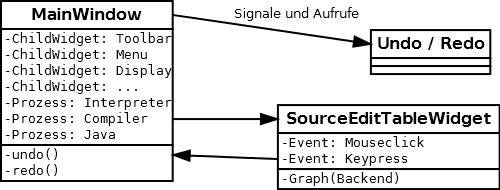
\includegraphics[width=0.7\textwidth]{editor-uebersicht}
	\end{figure}
\end{frame}


\section{Motivation}

\subsection{The Basic Problem That We Studied}

\begin{frame}{Make Titles Informative. Use Uppercase Letters. Long Titles are Split Automatically.}{Subtitles are optional.}
  % - A title should summarize the slide in an understandable fashion
  % for anyone how does not follow everything on the slide itself.
  \begin{itemize}
  \item
    Use \texttt{itemize} a lot.
  \item
    Use very short sentences or short phrases.
  \end{itemize}
\end{frame}

\begin{frame}{Make Titles Informative.}

  You can create overlays\dots
  \begin{itemize}
  \item using the \texttt{pause} command:
    \begin{itemize}
    \item
      First item.
      \pause
    \item
      Second item.
    \end{itemize}
  \item
    using overlay specifications:
    \begin{itemize}
    \item<3->
      First item.
    \item<4->
      Second item.
    \end{itemize}
  \item
    using the general \texttt{uncover} command:
    \begin{itemize}
      \uncover<5->{\item
        First item.}
      \uncover<6->{\item
        Second item.}
    \end{itemize}
  \end{itemize}
\end{frame}


\subsection{Previous Work}

\begin{frame}[fragile]{An old algorithm}
% NB. listings is quite powerful, but not well suited to be used with beamer
% consider using semiverbatim or the like, see below
\begin{lstlisting}[language=C]
int main (void)
{
  std::vector<bool> is_prime (100, true);
  for (int i = 2; i < 100; i++)
    if (is_prime[i])
      {
        std::cout << i << " ";
        for (int j = i; j < 100;
            is_prime [j] = false, j+=i);
      }
  return 0;
}
\end{lstlisting}
\end{frame}

\begin{frame}[fragile]
  \frametitle{An Algorithm For Finding Primes Numbers.}
\begin{semiverbatim}
\uncover<1->{\alert<0>{int main (void)}}
\uncover<1->{\alert<0>{\{}}
\uncover<1->{\alert<1>{ \alert<4>{std::}vector<bool> is_prime (100, true);}}
\uncover<1->{\alert<1>{ for (int i = 2; i < 100; i++)}}
\uncover<2->{\alert<2>{ if (is_prime[i])}}
\uncover<2->{\alert<0>{ \{}}
\uncover<3->{\alert<3>{ \alert<4>{std::}cout << i << " ";}}
\uncover<3->{\alert<3>{ for (int j = i; j < 100;}}
\uncover<3->{\alert<3>{ is_prime [j] = false, j+=i);}}
\uncover<2->{\alert<0>{ \}}}
\uncover<1->{\alert<0>{ return 0;}}
\uncover<1->{\alert<0>{\}}}
\end{semiverbatim}
  \visible<4->{Note the use of \alert{\texttt{std::}}.}
\end{frame}

\section{Our Results/Contribution}

\subsection{Main Results}

\begin{frame}{Make Titles Informative.}
  \begin{example}
    \begin{itemize}
    \item 2 is prime (two divisors: 1 and 2).
    \item 3 is prime (two divisors: 1 and 3).
    \item 4 is not prime (\alert{three} divisors: 1, 2, and 4).
    \end{itemize}
  \end{example}
\end{frame}

\begin{frame}{Make Titles Informative.}
\begin{theorem}
 There is no largest prime number and, in addition, $$\int_\Omega \nabla u \cdot \nabla v = - \int_\Omega u \Delta v + \int_{\partial\Omega} u v n$$
 \end{theorem}
 \begin{proof}
 \begin{enumerate}
 \item<1-> Suppose $p$ were the largest prime number.
 \item<2-> Let $q$ be the product of the first $p$ numbers.
 \item<3-> Then $q + 1$ is not divisible by any of them.
 \item<1-> Thus $q + 1$ is also prime and greater than $p$.\qedhere
 \end{enumerate}
 \end{proof}
 \uncover<4->{The proof used \textit{reductio ad absurdum}.}
\end{frame}

\begin{frame}{Make Titles Informative.}
\end{frame}


\subsection{Basic Ideas for Proofs/Implementation}

\begin{frame}{Make Titles Informative.}
\end{frame}

\begin{frame}{Make Titles Informative.}
\end{frame}

\begin{frame}{Make Titles Informative.}
\end{frame}



\section*{Summary}

\begin{frame}{Summary}

  % Keep the summary *very short*.
  \begin{itemize}
  \item
    The \alert{first main message} of your talk in one or two lines.
  \item
    The \alert{second main message} of your talk in one or two lines.
  \item
    Perhaps a \alert{third message}, but not more than that.
  \end{itemize}
  
  % The following outlook is optional.
  \vskip0pt plus.5fill
  \begin{itemize}
  \item
    Outlook
    \begin{itemize}
    \item
      Something you haven't solved.
    \item
      Something else you haven't solved.
    \end{itemize}
  \end{itemize}
\end{frame}



% All of the following is optional and typically not needed.
\appendix
\section<presentation>*{\appendixname}
\subsection<presentation>*{For Further Reading}

\begin{frame}[allowframebreaks]
  \frametitle<presentation>{For Further Reading}
    
  \begin{thebibliography}{10}
    
  \beamertemplatebookbibitems
  % Start with overview books.

  \bibitem{Author1990}
    A.~Author.
    \newblock {\em Handbook of Everything}.
    \newblock Some Press, 1990.
 
    
  \beamertemplatearticlebibitems
  % Followed by interesting articles. Keep the list short.

  \bibitem{Someone2000}
    S.~Someone.
    \newblock On this and that.
    \newblock {\em Journal of This and That}, 2(1):50--100,
    2000.
  \end{thebibliography}
\end{frame}

\end{document}
